\chapter{Experimental results}\label{ch:experiment}

In this chapter we present the results of experiments, conducted in lab
environment, against two major systems, Facebook Chat and Gmail. We will analyze
the validity of the attack under different modes, serial and parallel, as well
as the time consumption of each method. Also, we will investigate the
effectiveness of the point-system meta-predictor, introduced in Section
\ref{subsec:point_system}.

\section{Facebook Chat messages}\label{sec:fb_experiment}

The first experiment targeted Facebook Chat, trying to exploit the vulnerability
presented in Section \ref{subsec:fb}. The first attempt used a regulat Facebook
account, with hundreds of friends and regular chat conversations and
notifications. However, using the validation method of Section
\ref{sec:mitmproxy}, it was found that between the secret and the reflection
lied a large amount of data, which led to a non-compression of the two, since
the LZ77 was not sufficient.

For that matter of this paper we have created a lab account, that has no friends
and no user activity of any kind, except for a self-sent private message, that
will be the secret to be stolen. That way, the noise of a real-world account,
such as new messages or notifications, is contained and we can avoid the
problems described above.

We assume an attack on Facebook chat messages, following the serial method of
requests, knowing the secret consists of letters, either lowercase or uppercase.
In order to steal the first letter of the secret, we perform 4000 iterations of
requests, which translates to 4000 for each letter in the alphabet or, in other
words, \begin{math}4000*52=208000\end{math} requests in total. The normal time
interval between two requests was set to 4 seconds, in order to be sure that
overlapping stream can be distinguished. This has led to an overall
\begin{math}208000*4 = 832000\end{math} seconds, which roughly equals to 9 days.

The following figure shows the behaviour of the correct letter as the attack
evolved:

\begin{figure}[H] \caption{Correct letter length chart.}
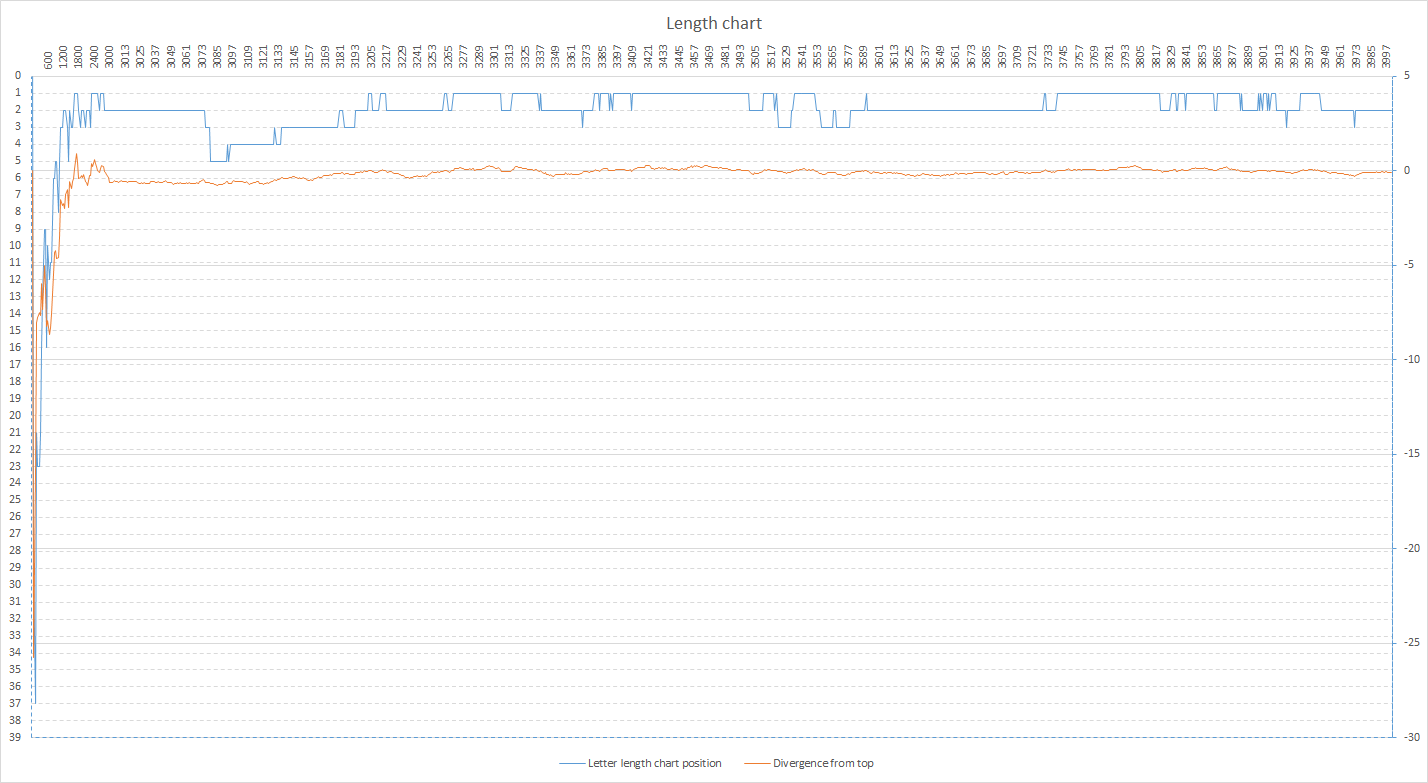
\includegraphics[width=1\textwidth]{diagrams/point_system_chart_1.png}\end{figure}

The top horizontal axis contains the number of iterations of requests.

The left vertical axis shows the position of the correct letter compared to the
others in ascending mean length order, i.e. the letter with minimum mean length
is \texttt{1}, the second smaller is \texttt{2} etc, and corresponds to the blue
curve.

The right vertical axis depicts the difference of the mean lengths of the
correct letter and the \textit{best} one, i.e. the one with minimum mean length,
or the second \textit{best}, in case the correct letter is the one of minimum
mean length.  This corresponds to the orange curve.

It can be understood that the correct guess presents a good behaviour after a
transient period, however, it does not always respond to the minimum mean
response length. In order to handle this problem, we introduced the point-system meta-predictor,
presented in Section \ref{subsec:point_system}. In a similar manner, we parsed
the collected data, using the point-system information.

The chart depicting the evolution of the correct letter's
behaviour in time, regarding the aggregated points, is shown in the following
figure:

\begin{figure}[H] \caption{Correct letter point chart.}
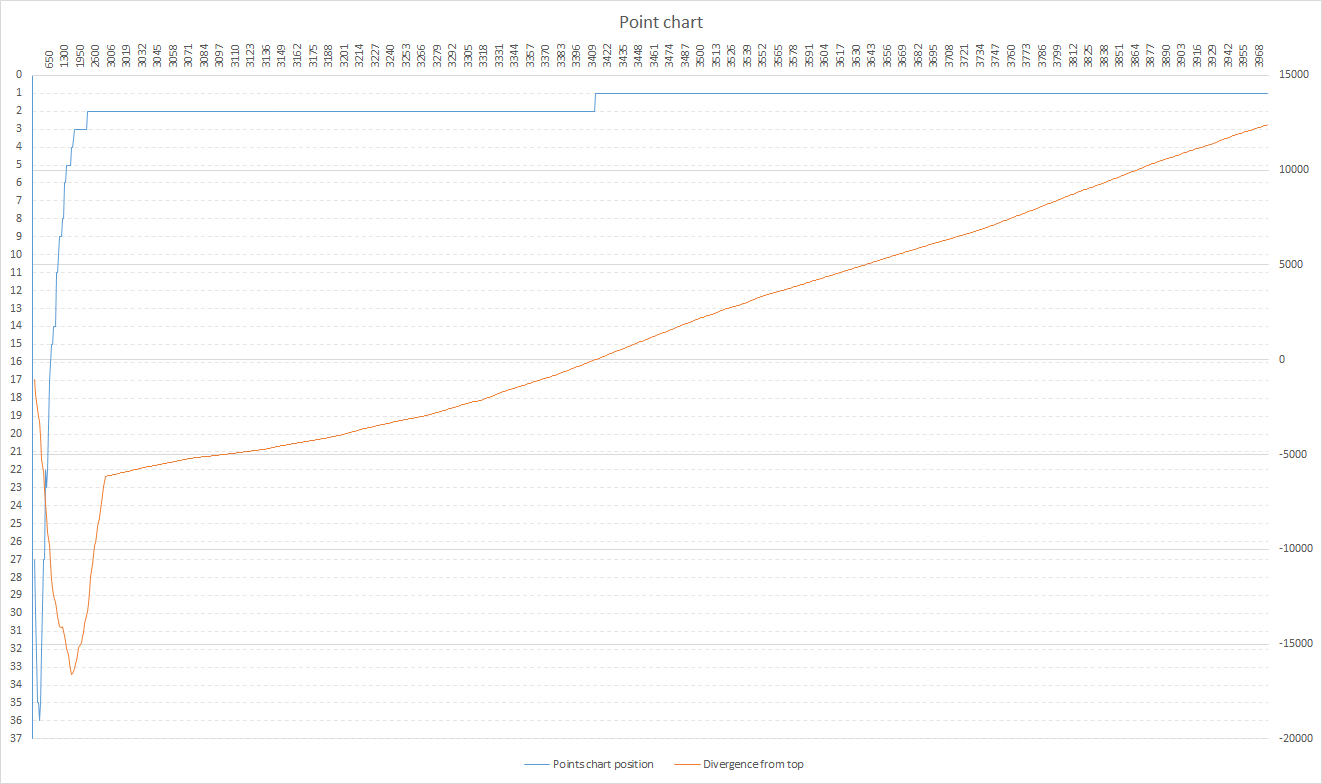
\includegraphics[width=1\textwidth]{diagrams/point_system_chart_2.png}\end{figure}

It is clear that, by introducing the point system, the prediction of the correct
letter is much more efficient than before. After a transient period, the correct
letter demonstrates a better behaviour compared to any other choice, increasing
its point performance in an almost linear rate over time.

The demonstrated attack provides a statistical proof that Facebook Chat is not
IND-PCPA. It is clear that an adversary could gain a major advantage in stealing a
private Facebook Chat message, using this attack model. However, it can be
understood that the attack performance of the attack is very limited, making it
particularly hard to be applied in real-world, where the conditions for success
would need to be applied for a noticeable period of time.

\section{Gmail Authentication token}\label{sec:gmail_experiment}


